\pgfdeclareplotmark{cross} {
\pgfpathmoveto{\pgfpoint{-0.3\pgfplotmarksize}{\pgfplotmarksize}}
\pgfpathlineto{\pgfpoint{+0.3\pgfplotmarksize}{\pgfplotmarksize}}
\pgfpathlineto{\pgfpoint{+0.3\pgfplotmarksize}{0.3\pgfplotmarksize}}
\pgfpathlineto{\pgfpoint{+1\pgfplotmarksize}{0.3\pgfplotmarksize}}
\pgfpathlineto{\pgfpoint{+1\pgfplotmarksize}{-0.3\pgfplotmarksize}}
\pgfpathlineto{\pgfpoint{+0.3\pgfplotmarksize}{-0.3\pgfplotmarksize}}
\pgfpathlineto{\pgfpoint{+0.3\pgfplotmarksize}{-1.\pgfplotmarksize}}
\pgfpathlineto{\pgfpoint{-0.3\pgfplotmarksize}{-1.\pgfplotmarksize}}
\pgfpathlineto{\pgfpoint{-0.3\pgfplotmarksize}{-0.3\pgfplotmarksize}}
\pgfpathlineto{\pgfpoint{-1.\pgfplotmarksize}{-0.3\pgfplotmarksize}}
\pgfpathlineto{\pgfpoint{-1.\pgfplotmarksize}{0.3\pgfplotmarksize}}
\pgfpathlineto{\pgfpoint{-0.3\pgfplotmarksize}{0.3\pgfplotmarksize}}
\pgfpathclose
\pgfusepathqstroke
}
\pgfdeclareplotmark{cross*} {
\pgfpathmoveto{\pgfpoint{-0.3\pgfplotmarksize}{\pgfplotmarksize}}
\pgfpathlineto{\pgfpoint{+0.3\pgfplotmarksize}{\pgfplotmarksize}}
\pgfpathlineto{\pgfpoint{+0.3\pgfplotmarksize}{0.3\pgfplotmarksize}}
\pgfpathlineto{\pgfpoint{+1\pgfplotmarksize}{0.3\pgfplotmarksize}}
\pgfpathlineto{\pgfpoint{+1\pgfplotmarksize}{-0.3\pgfplotmarksize}}
\pgfpathlineto{\pgfpoint{+0.3\pgfplotmarksize}{-0.3\pgfplotmarksize}}
\pgfpathlineto{\pgfpoint{+0.3\pgfplotmarksize}{-1.\pgfplotmarksize}}
\pgfpathlineto{\pgfpoint{-0.3\pgfplotmarksize}{-1.\pgfplotmarksize}}
\pgfpathlineto{\pgfpoint{-0.3\pgfplotmarksize}{-0.3\pgfplotmarksize}}
\pgfpathlineto{\pgfpoint{-1.\pgfplotmarksize}{-0.3\pgfplotmarksize}}
\pgfpathlineto{\pgfpoint{-1.\pgfplotmarksize}{0.3\pgfplotmarksize}}
\pgfpathlineto{\pgfpoint{-0.3\pgfplotmarksize}{0.3\pgfplotmarksize}}
\pgfpathclose
\pgfusepathqfillstroke
}
\pgfdeclareplotmark{newstar} {
\pgfpathmoveto{\pgfqpoint{0pt}{\pgfplotmarksize}}
\pgfpathlineto{\pgfqpointpolar{44}{0.5\pgfplotmarksize}}
\pgfpathlineto{\pgfqpointpolar{18}{\pgfplotmarksize}}
\pgfpathlineto{\pgfqpointpolar{-20}{0.5\pgfplotmarksize}}
\pgfpathlineto{\pgfqpointpolar{-54}{\pgfplotmarksize}}
\pgfpathlineto{\pgfqpointpolar{-90}{0.5\pgfplotmarksize}}
\pgfpathlineto{\pgfqpointpolar{234}{\pgfplotmarksize}}
\pgfpathlineto{\pgfqpointpolar{198}{0.5\pgfplotmarksize}}
\pgfpathlineto{\pgfqpointpolar{162}{\pgfplotmarksize}}
\pgfpathlineto{\pgfqpointpolar{134}{0.5\pgfplotmarksize}}
\pgfpathclose
\pgfusepathqstroke
}
\pgfdeclareplotmark{newstar*} {
\pgfpathmoveto{\pgfqpoint{0pt}{\pgfplotmarksize}}
\pgfpathlineto{\pgfqpointpolar{44}{0.5\pgfplotmarksize}}
\pgfpathlineto{\pgfqpointpolar{18}{\pgfplotmarksize}}
\pgfpathlineto{\pgfqpointpolar{-20}{0.5\pgfplotmarksize}}
\pgfpathlineto{\pgfqpointpolar{-54}{\pgfplotmarksize}}
\pgfpathlineto{\pgfqpointpolar{-90}{0.5\pgfplotmarksize}}
\pgfpathlineto{\pgfqpointpolar{234}{\pgfplotmarksize}}
\pgfpathlineto{\pgfqpointpolar{198}{0.5\pgfplotmarksize}}
\pgfpathlineto{\pgfqpointpolar{162}{\pgfplotmarksize}}
\pgfpathlineto{\pgfqpointpolar{134}{0.5\pgfplotmarksize}}
\pgfpathclose
\pgfusepathqfillstroke
}
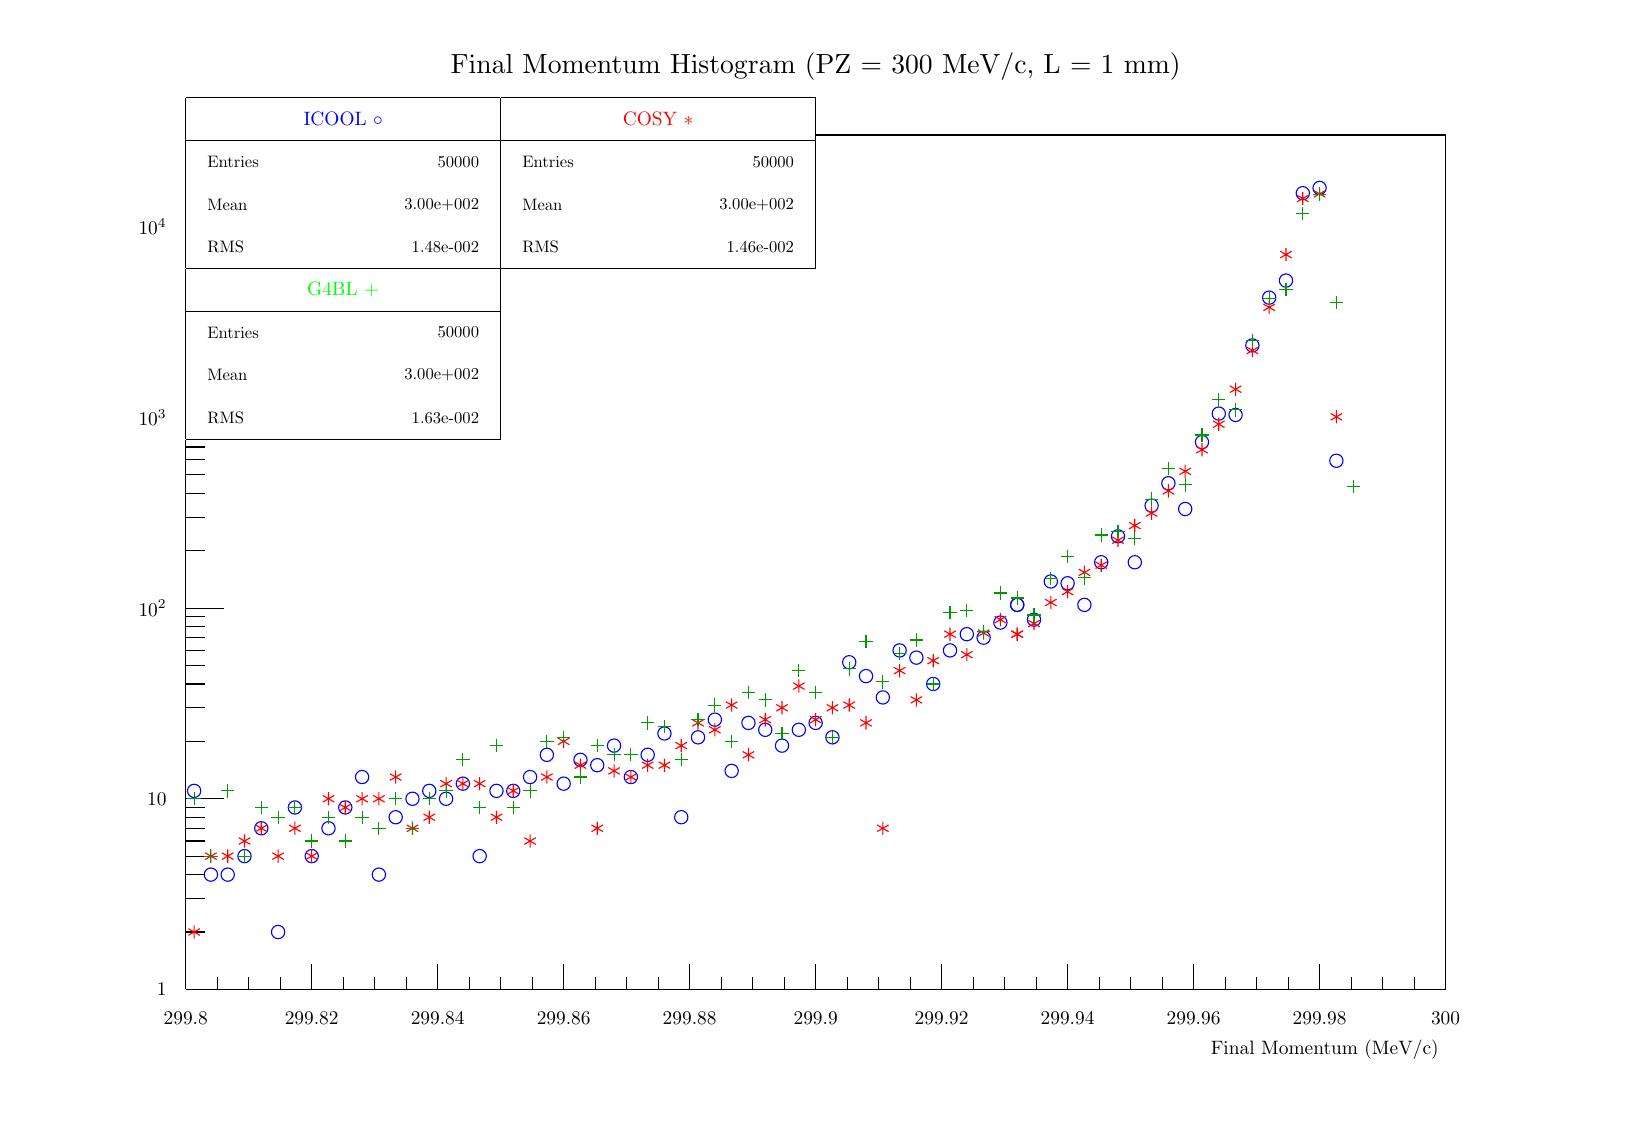
\begin{tikzpicture}
\definecolor{c}{rgb}{1,1,1};
\draw [color=c, fill=c] (0,0) rectangle (20,13.5632);
\draw [color=c, fill=c] (2,1.35632) rectangle (18,12.2069);
\definecolor{c}{rgb}{0,0,0};
\draw [c] (2,1.35632) -- (2,12.2069) -- (18,12.2069) -- (18,1.35632) -- (2,1.35632);
\definecolor{c}{rgb}{1,1,1};
\draw [color=c, fill=c] (2,1.35632) rectangle (18,12.2069);
\definecolor{c}{rgb}{0,0,0};
\draw [c] (2,1.35632) -- (2,12.2069) -- (18,12.2069) -- (18,1.35632) -- (2,1.35632);
\definecolor{c}{rgb}{0,0,1};
\foreach \P in
 {(2.10667,3.87762),(2.32,2.81396),(2.53333,2.81396),(2.74667,3.04859),(2.96,3.40238),(3.17333,2.08514),(3.38667,3.66663),(3.6,3.04859),(3.81333,3.40238),(4.02667,3.66663),(4.24,4.05328),(4.45333,2.81396),(4.66667,3.54278),(4.88,3.77741),(5.09333,3.8
7762),(5.30667,3.77741),(5.52,3.96911),(5.73333,3.04859),(5.94667,3.87762),(6.16,3.87762),(6.37333,4.05328),(6.58667,4.33535),(6.8,3.96911),(7.01333,4.2716),(7.22667,4.20374),(7.44,4.4523),(7.65333,4.05328),(7.86667,4.33535),(8.08,4.60644),(8.29333,3
.54278),(8.50667,4.55753),(8.72,4.78209),(8.93333,4.1312),(9.14667,4.74086),(9.36,4.65318),(9.57333,4.4523),(9.78667,4.65318),(10,4.74086),(10.2133,4.55753),(10.4267,5.51091),(10.64,5.33526),(10.8533,5.06417),(11.0667,5.66138),(11.28,5.56989),(11.493
3,5.23505),(11.7067,5.66138),(11.92,5.86759),(12.1333,5.82346),(12.3467,6.01517),(12.56,6.23973)}{\draw[mark options={color=c,fill=c},mark size=2.402402pt,mark=o] plot coordinates {\P};}
\foreach \P in
 {(12.56,6.23973),(12.7733,6.05207),(12.9867,6.53715),(13.2,6.51404),(13.4133,6.23973),(13.6267,6.78089),(13.84,7.11022),(14.0533,6.78089),(14.2667,7.5006),(14.48,7.78464),(14.6933,7.45704),(14.9067,8.30723),(15.12,8.66888),(15.3333,8.65168),(15.5467
,9.53484),(15.76,10.1417),(15.9733,10.3585),(16.1867,11.4676),(16.4,11.5349),(16.6133,8.07013)}{\draw[mark options={color=c,fill=c},mark size=2.402402pt,mark=o] plot coordinates {\P};}
\definecolor{c}{rgb}{1,1,1};
\draw [color=c, fill=c] (2,10.5115) rectangle (6,12.6816);
\definecolor{c}{rgb}{0,0,0};
\draw [c] (2,10.5115) -- (6,10.5115);
\draw [c] (6,10.5115) -- (6,12.6816);
\draw [c] (6,12.6816) -- (2,12.6816);
\draw [c] (2,12.6816) -- (2,10.5115);
\draw[color=blue](4,12.4103) node[scale=0.7, rotate=0]{ICOOL $\circ$};
\draw [c] (2,12.1391) -- (6,12.1391);
\draw [anchor= west] (2.2,11.8678) node[scale=0.6, rotate=0]{Entries };
\draw [anchor= east] (5.8,11.8678) node[scale=0.6, rotate=0]{ 50000};
\draw [anchor= west] (2.2,11.3253) node[scale=0.6, rotate=0]{Mean  };
\draw [anchor= east] (5.8,11.3253) node[scale=0.6, rotate=0]{ 3.00e+002};
\draw [anchor= west] (2.2,10.7828) node[scale=0.6, rotate=0]{RMS   };
\draw [anchor= east] (5.8,10.7828) node[scale=0.6, rotate=0]{ 1.48e-002};
\draw [c] (2,1.35632) -- (18,1.35632);
\draw [anchor= east] (18,0.596782) node[scale=0.7, rotate=0]{Final Momentum (MeV/c)};
\draw [c] (2,1.68184) -- (2,1.35632);
\draw [c] (2.4,1.51908) -- (2.4,1.35632);
\draw [c] (2.8,1.51908) -- (2.8,1.35632);
\draw [c] (3.2,1.51908) -- (3.2,1.35632);
\draw [c] (3.6,1.68184) -- (3.6,1.35632);
\draw [c] (4,1.51908) -- (4,1.35632);
\draw [c] (4.4,1.51908) -- (4.4,1.35632);
\draw [c] (4.8,1.51908) -- (4.8,1.35632);
\draw [c] (5.2,1.68184) -- (5.2,1.35632);
\draw [c] (5.6,1.51908) -- (5.6,1.35632);
\draw [c] (6,1.51908) -- (6,1.35632);
\draw [c] (6.4,1.51908) -- (6.4,1.35632);
\draw [c] (6.8,1.68184) -- (6.8,1.35632);
\draw [c] (7.2,1.51908) -- (7.2,1.35632);
\draw [c] (7.6,1.51908) -- (7.6,1.35632);
\draw [c] (8,1.51908) -- (8,1.35632);
\draw [c] (8.4,1.68184) -- (8.4,1.35632);
\draw [c] (8.8,1.51908) -- (8.8,1.35632);
\draw [c] (9.2,1.51908) -- (9.2,1.35632);
\draw [c] (9.6,1.51908) -- (9.6,1.35632);
\draw [c] (10,1.68184) -- (10,1.35632);
\draw [c] (10.4,1.51908) -- (10.4,1.35632);
\draw [c] (10.8,1.51908) -- (10.8,1.35632);
\draw [c] (11.2,1.51908) -- (11.2,1.35632);
\draw [c] (11.6,1.68184) -- (11.6,1.35632);
\draw [c] (12,1.51908) -- (12,1.35632);
\draw [c] (12.4,1.51908) -- (12.4,1.35632);
\draw [c] (12.8,1.51908) -- (12.8,1.35632);
\draw [c] (13.2,1.68184) -- (13.2,1.35632);
\draw [c] (13.6,1.51908) -- (13.6,1.35632);
\draw [c] (14,1.51908) -- (14,1.35632);
\draw [c] (14.4,1.51908) -- (14.4,1.35632);
\draw [c] (14.8,1.68184) -- (14.8,1.35632);
\draw [c] (15.2,1.51908) -- (15.2,1.35632);
\draw [c] (15.6,1.51908) -- (15.6,1.35632);
\draw [c] (16,1.51908) -- (16,1.35632);
\draw [c] (16.4,1.68184) -- (16.4,1.35632);
\draw [c] (16.8,1.51908) -- (16.8,1.35632);
\draw [c] (17.2,1.51908) -- (17.2,1.35632);
\draw [c] (17.6,1.51908) -- (17.6,1.35632);
\draw [c] (18,1.68184) -- (18,1.35632);
\draw [anchor=base] (2,0.908736) node[scale=0.7, rotate=0]{299.8};
\draw [anchor=base] (3.6,0.908736) node[scale=0.7, rotate=0]{299.82};
\draw [anchor=base] (5.2,0.908736) node[scale=0.7, rotate=0]{299.84};
\draw [anchor=base] (6.8,0.908736) node[scale=0.7, rotate=0]{299.86};
\draw [anchor=base] (8.4,0.908736) node[scale=0.7, rotate=0]{299.88};
\draw [anchor=base] (10,0.908736) node[scale=0.7, rotate=0]{299.9};
\draw [anchor=base] (11.6,0.908736) node[scale=0.7, rotate=0]{299.92};
\draw [anchor=base] (13.2,0.908736) node[scale=0.7, rotate=0]{299.94};
\draw [anchor=base] (14.8,0.908736) node[scale=0.7, rotate=0]{299.96};
\draw [anchor=base] (16.4,0.908736) node[scale=0.7, rotate=0]{299.98};
\draw [anchor=base] (18,0.908736) node[scale=0.7, rotate=0]{300};
\draw [c] (2,1.35632) -- (2,12.2069);
\draw [c] (2.48,1.35632) -- (2,1.35632);
\draw [anchor= east] (1.844,1.35632) node[scale=0.7, rotate=0]{1};
\draw [c] (2.24,2.08514) -- (2,2.08514);
\draw [c] (2.24,2.51148) -- (2,2.51148);
\draw [c] (2.24,2.81396) -- (2,2.81396);
\draw [c] (2.24,3.04859) -- (2,3.04859);
\draw [c] (2.24,3.2403) -- (2,3.2403);
\draw [c] (2.24,3.40238) -- (2,3.40238);
\draw [c] (2.24,3.54278) -- (2,3.54278);
\draw [c] (2.24,3.66663) -- (2,3.66663);
\draw [c] (2.48,3.77741) -- (2,3.77741);
\draw [anchor= east] (1.844,3.77741) node[scale=0.7, rotate=0]{10};
\draw [c] (2.24,4.50623) -- (2,4.50623);
\draw [c] (2.24,4.93256) -- (2,4.93256);
\draw [c] (2.24,5.23505) -- (2,5.23505);
\draw [c] (2.24,5.46968) -- (2,5.46968);
\draw [c] (2.24,5.66138) -- (2,5.66138);
\draw [c] (2.24,5.82347) -- (2,5.82347);
\draw [c] (2.24,5.96387) -- (2,5.96387);
\draw [c] (2.24,6.08771) -- (2,6.08771);
\draw [c] (2.48,6.1985) -- (2,6.1985);
\draw [anchor= east] (1.844,6.1985) node[scale=0.7, rotate=0]{$10^{2}$};
\draw [c] (2.24,6.92732) -- (2,6.92732);
\draw [c] (2.24,7.35365) -- (2,7.35365);
\draw [c] (2.24,7.65614) -- (2,7.65614);
\draw [c] (2.24,7.89076) -- (2,7.89076);
\draw [c] (2.24,8.08247) -- (2,8.08247);
\draw [c] (2.24,8.24455) -- (2,8.24455);
\draw [c] (2.24,8.38496) -- (2,8.38496);
\draw [c] (2.24,8.5088) -- (2,8.5088);
\draw [c] (2.48,8.61958) -- (2,8.61958);
\draw [anchor= east] (1.844,8.61958) node[scale=0.7, rotate=0]{$10^{3}$};
\draw [c] (2.24,9.3484) -- (2,9.3484);
\draw [c] (2.24,9.77473) -- (2,9.77473);
\draw [c] (2.24,10.0772) -- (2,10.0772);
\draw [c] (2.24,10.3118) -- (2,10.3118);
\draw [c] (2.24,10.5036) -- (2,10.5036);
\draw [c] (2.24,10.6656) -- (2,10.6656);
\draw [c] (2.24,10.806) -- (2,10.806);
\draw [c] (2.24,10.9299) -- (2,10.9299);
\draw [c] (2.48,11.0407) -- (2,11.0407);
\draw [anchor= east] (1.844,11.0407) node[scale=0.7, rotate=0]{$10^{4}$};
\draw [c] (2.24,11.7695) -- (2,11.7695);
\draw [c] (2.24,12.1958) -- (2,12.1958);
\definecolor{c}{rgb}{1,1,1};
\draw [color=c, fill=c] (2,10.5115) rectangle (6,12.6816);
\definecolor{c}{rgb}{0,0,0};
\draw [c] (2,10.5115) -- (6,10.5115);
\draw [c] (6,10.5115) -- (6,12.6816);
\draw [c] (6,12.6816) -- (2,12.6816);
\draw [c] (2,12.6816) -- (2,10.5115);
\draw[color=blue](4,12.4103) node[scale=0.7, rotate=0]{ICOOL $\circ$};
\draw [c] (2,12.1391) -- (6,12.1391);
\draw [anchor= west] (2.2,11.8678) node[scale=0.6, rotate=0]{Entries };
\draw [anchor= east] (5.8,11.8678) node[scale=0.6, rotate=0]{ 50000};
\draw [anchor= west] (2.2,11.3253) node[scale=0.6, rotate=0]{Mean  };
\draw [anchor= east] (5.8,11.3253) node[scale=0.6, rotate=0]{ 3.00e+002};
\draw [anchor= west] (2.2,10.7828) node[scale=0.6, rotate=0]{RMS   };
\draw [anchor= east] (5.8,10.7828) node[scale=0.6, rotate=0]{ 1.48e-002};
\draw (10,13.0816) node[scale=1, rotate=0]{Final Momentum Histogram (PZ = 300 MeV/c, L = 1 mm)};
\definecolor{c}{rgb}{1,0,0};
\foreach \P in
 {(2.10667,2.08514),(2.32,3.04859),(2.53333,3.04859),(2.74667,3.24029),(2.96,3.40238),(3.17333,3.04859),(3.38667,3.40238),(3.6,3.04859),(3.81333,3.77741),(4.02667,3.66663),(4.24,3.77741),(4.45333,3.77741),(4.66667,4.05328),(4.88,3.40238),(5.09333,3.5
4278),(5.30667,3.96911),(5.52,3.96911),(5.73333,3.96911),(5.94667,3.54278),(6.16,3.87762),(6.37333,3.24029),(6.58667,4.05328),(6.8,4.50623),(7.01333,4.20374),(7.22667,3.40238),(7.44,4.1312),(7.65333,4.05328),(7.86667,4.20374),(8.08,4.20374),(8.29333,
4.4523),(8.50667,4.74086),(8.72,4.65318),(8.93333,4.96704),(9.14667,4.33535),(9.36,4.78209),(9.57333,4.93256),(9.78667,5.20843),(10,4.78209),(10.2133,4.93256),(10.4267,4.96704),(10.64,4.74086),(10.8533,3.40238),(11.0667,5.40462),(11.28,5.03278),(11.4
933,5.53094),(11.7067,5.86759),(11.92,5.60745),(12.1333,5.88189),(12.3467,6.05207),(12.56,5.86759)}{\draw[mark options={color=c,fill=c},mark size=2.402402pt,mark=asterisk] plot coordinates {\P};}
\foreach \P in
 {(12.56,5.86759),(12.7733,6.00258),(12.9867,6.26964),(13.2,6.40758),(13.4133,6.6525),(13.6267,6.74399),(13.84,7.06046),(14.0533,7.24675),(14.2667,7.40495),(14.48,7.68721),(14.6933,7.93604),(14.9067,8.20942),(15.12,8.53419),(15.3333,8.97861),(15.5467
,9.46991),(15.76,10.0186),(15.9733,10.6882),(16.1867,11.4008),(16.4,11.4593),(16.6133,8.62796)}{\draw[mark options={color=c,fill=c},mark size=2.402402pt,mark=asterisk] plot coordinates {\P};}
\definecolor{c}{rgb}{1,1,1};
\draw [color=c, fill=c] (6,10.5115) rectangle (10,12.6816);
\definecolor{c}{rgb}{0,0,0};
\draw [c] (6,10.5115) -- (10,10.5115);
\draw [c] (10,10.5115) -- (10,12.6816);
\draw [c] (10,12.6816) -- (6,12.6816);
\draw [c] (6,12.6816) -- (6,10.5115);
\draw [color=red](8,12.4103) node[scale=0.7, rotate=0]{COSY $*$};
\draw [c] (6,12.1391) -- (10,12.1391);
\draw [anchor= west] (6.2,11.8678) node[scale=0.6, rotate=0]{Entries };
\draw [anchor= east] (9.8,11.8678) node[scale=0.6, rotate=0]{ 50000};
\draw [anchor= west] (6.2,11.3253) node[scale=0.6, rotate=0]{Mean  };
\draw [anchor= east] (9.8,11.3253) node[scale=0.6, rotate=0]{ 3.00e+002};
\draw [anchor= west] (6.2,10.7828) node[scale=0.6, rotate=0]{RMS   };
\draw [anchor= east] (9.8,10.7828) node[scale=0.6, rotate=0]{ 1.46e-002};
\definecolor{c}{rgb}{1,1,1};
\draw [color=c, fill=c] (6,10.5115) rectangle (10,12.6816);
\definecolor{c}{rgb}{0,0,0};
\draw [c] (6,10.5115) -- (10,10.5115);
\draw [c] (10,10.5115) -- (10,12.6816);
\draw [c] (10,12.6816) -- (6,12.6816);
\draw [c] (6,12.6816) -- (6,10.5115);
\draw [color=red](8,12.4103) node[scale=0.7, rotate=0]{COSY $*$};
\draw [c] (6,12.1391) -- (10,12.1391);
\draw [anchor= west] (6.2,11.8678) node[scale=0.6, rotate=0]{Entries };
\draw [anchor= east] (9.8,11.8678) node[scale=0.6, rotate=0]{ 50000};
\draw [anchor= west] (6.2,11.3253) node[scale=0.6, rotate=0]{Mean  };
\draw [anchor= east] (9.8,11.3253) node[scale=0.6, rotate=0]{ 3.00e+002};
\draw [anchor= west] (6.2,10.7828) node[scale=0.6, rotate=0]{RMS   };
\draw [anchor= east] (9.8,10.7828) node[scale=0.6, rotate=0]{ 1.46e-002};
\definecolor{c}{rgb}{0,0.6,0};
\foreach \P in
 {(2.10667,3.77741),(2.32,3.04859),(2.53333,3.87762),(2.74667,3.04859),(2.96,3.66663),(3.17333,3.54278),(3.38667,3.66663),(3.6,3.24029),(3.81333,3.54278),(4.02667,3.24029),(4.24,3.54278),(4.45333,3.40238),(4.66667,3.77741),(4.88,3.40238),(5.09333,3.7
7741),(5.30667,3.87762),(5.52,4.2716),(5.73333,3.66663),(5.94667,4.4523),(6.16,3.66663),(6.37333,3.87762),(6.58667,4.50623),(6.8,4.55753),(7.01333,4.05328),(7.22667,4.4523),(7.44,4.33535),(7.65333,4.33535),(7.86667,4.74086),(8.08,4.69793),(8.29333,4.
2716),(8.50667,4.78209),(8.72,4.96704),(8.93333,4.50623),(9.14667,5.12427),(9.36,5.03278),(9.57333,4.60644),(9.78667,5.40462),(10,5.12427),(10.2133,4.55753),(10.4267,5.42675),(10.64,5.77741),(10.8533,5.26101),(11.0667,5.62573),(11.28,5.79298),(11.493
3,5.23505),(11.7067,6.14456),(11.92,6.16647),(12.1333,5.89601),(12.3467,6.3902),(12.56,6.327)}{\draw[mark options={color=c,fill=c},mark size=2.402402pt,mark=+] plot coordinates {\P};}
\foreach \P in
 {(12.56,6.327),(12.7733,6.11082),(12.9867,6.57458),(13.2,6.85665),(13.4133,6.5819),(13.6267,7.12775),(13.84,7.17032),(14.0533,7.07883),(14.2667,7.58265),(14.48,7.96778),(14.6933,7.76349),(14.9067,8.39672),(15.12,8.84746),(15.3333,8.71597),(15.5467,9
.5964),(15.76,10.1345),(15.9733,10.245),(16.1867,11.213),(16.4,11.4477),(16.6133,10.0838),(16.8267,7.74191)}{\draw[mark options={color=c,fill=c},mark size=2.402402pt,mark=+] plot coordinates {\P};}
\definecolor{c}{rgb}{1,1,1};
\draw [color=c, fill=c] (2,8.34138) rectangle (6,10.5115);
\definecolor{c}{rgb}{0,0,0};
\draw [c] (2,8.34138) -- (6,8.34138);
\draw [c] (6,8.34138) -- (6,10.5115);
\draw [c] (6,10.5115) -- (2,10.5115);
\draw [c] (2,10.5115) -- (2,8.34138);
\draw [color=green](4,10.2402) node[scale=0.7, rotate=0]{G4BL $+$};
\draw [c] (2,9.96897) -- (6,9.96897);
\draw [anchor= west] (2.2,9.6977) node[scale=0.6, rotate=0]{Entries };
\draw [anchor= east] (5.8,9.6977) node[scale=0.6, rotate=0]{ 50000};
\draw [anchor= west] (2.2,9.15517) node[scale=0.6, rotate=0]{Mean  };
\draw [anchor= east] (5.8,9.15517) node[scale=0.6, rotate=0]{ 3.00e+002};
\draw [anchor= west] (2.2,8.61264) node[scale=0.6, rotate=0]{RMS   };
\draw [anchor= east] (5.8,8.61264) node[scale=0.6, rotate=0]{ 1.63e-002};
\definecolor{c}{rgb}{1,1,1};
\draw [color=c, fill=c] (2,8.34138) rectangle (6,10.5115);
\definecolor{c}{rgb}{0,0,0};
\draw [c] (2,8.34138) -- (6,8.34138);
\draw [c] (6,8.34138) -- (6,10.5115);
\draw [c] (6,10.5115) -- (2,10.5115);
\draw [c] (2,10.5115) -- (2,8.34138);
\draw [color=green](4,10.2402) node[scale=0.7, rotate=0]{G4BL $+$};
\draw [c] (2,9.96897) -- (6,9.96897);
\draw [anchor= west] (2.2,9.6977) node[scale=0.6, rotate=0]{Entries };
\draw [anchor= east] (5.8,9.6977) node[scale=0.6, rotate=0]{ 50000};
\draw [anchor= west] (2.2,9.15517) node[scale=0.6, rotate=0]{Mean  };
\draw [anchor= east] (5.8,9.15517) node[scale=0.6, rotate=0]{ 3.00e+002};
\draw [anchor= west] (2.2,8.61264) node[scale=0.6, rotate=0]{RMS   };
\draw [anchor= east] (5.8,8.61264) node[scale=0.6, rotate=0]{ 1.63e-002};
\end{tikzpicture}
